% Note: this file can be compiled on its own, but is also included by
% diss.tex (using the docmute.sty package to ignore the preamble)
\documentclass[12pt,a4paper,twoside]{article}
\usepackage[pdfborder={0 0 0}]{hyperref}
\usepackage[margin=25mm]{geometry}
\usepackage{graphicx}
\usepackage{parskip}
\usepackage{amssymb}
% \hypersetup{
%     colorlinks=false,
%     linkcolor=blue,
%     filecolor=magenta,      
%     urlcolor=blue,
% }
\begin{document}

\begin{center}
\Large
Computer Science Tripos -- Part II Project\\[4mm]
\LARGE
User Study Plan \\[4mm]

\large
George Andersen, gla23, Robinson College

\today

\end{center}

\vspace{5mm}

% Main Document
\section*{Data collection}
Aim to get qualitative and quantitative data that can be used in the evaluation.
The data will be collected in three sections

\begin{enumerate}
	\item Qualitative questionnaire

	First the users will asked a questionnaire

	\begin{enumerate}
		\item Have you ever played the game QWOP before?

		$\square$ Yes

		$\square$ No

		If so, how long have you played it for?

		$\square$ less that 5 minutes

		$\square$ Between 5 and 30 minutes

		$\square$ More than 30 minutes

		could add other questions like how far do you remember travelling, did you enjoy it, etc
		%\mbox{\ooalign{$\checkmark$\cr\hidewidth$\square$\hidewidth\cr}}

		% \item something else
	\end{enumerate}

	\item Game test

	Then the users will be split into two groups, A and B. Each user in group A will be moved on to another screen where they are instructed to play the original game of QWOP for 10 (too long?) minutes. After the time is up, the users will be moved on to my version which they will play for the same amount of time. The users in group B will do the same but with the orderings of the versions reversed.

	During this time data will be collected, such as:

	\begin{enumerate}
		\item Keys pressed

		Can use a key logger to record all the key presses the user makes. 
		Need to investigate how to do that, and also how to get the original qwop to be embedded in the test.
		\item Distance travelled 

		record the distance the user managed to travel for each run during the playtime, also with whether the athlete falls over or the user restarted.
		\item Screen capture?

		Since the data for the original qwop can't be collected through the game (again need to investigate how much I can access of the original) I should record the video of the player playing, then I can get data (e.g. distance travelled) from the video afterwards?

		Could also investigate qwopper or the method used in the qwop gaits paper to work out the distances as they play.

		10 minute video 600 MB
	\end{enumerate}

	This data would be stored in the area I'm hosting the test

	\item Final questionnaire
	After the users play the versions, there would be another questionnaire asking other questions:

	\begin{enumerate}
		\item Which version do you think you were more successful at?
		\item Which version felt like you had more control over the athlete?
		\item Do you think that playing the first version first meant your scores for the second one improved?
		\item Which version of the game did you enjoy most?
		\item 
	\end{enumerate}



\end{enumerate}

% 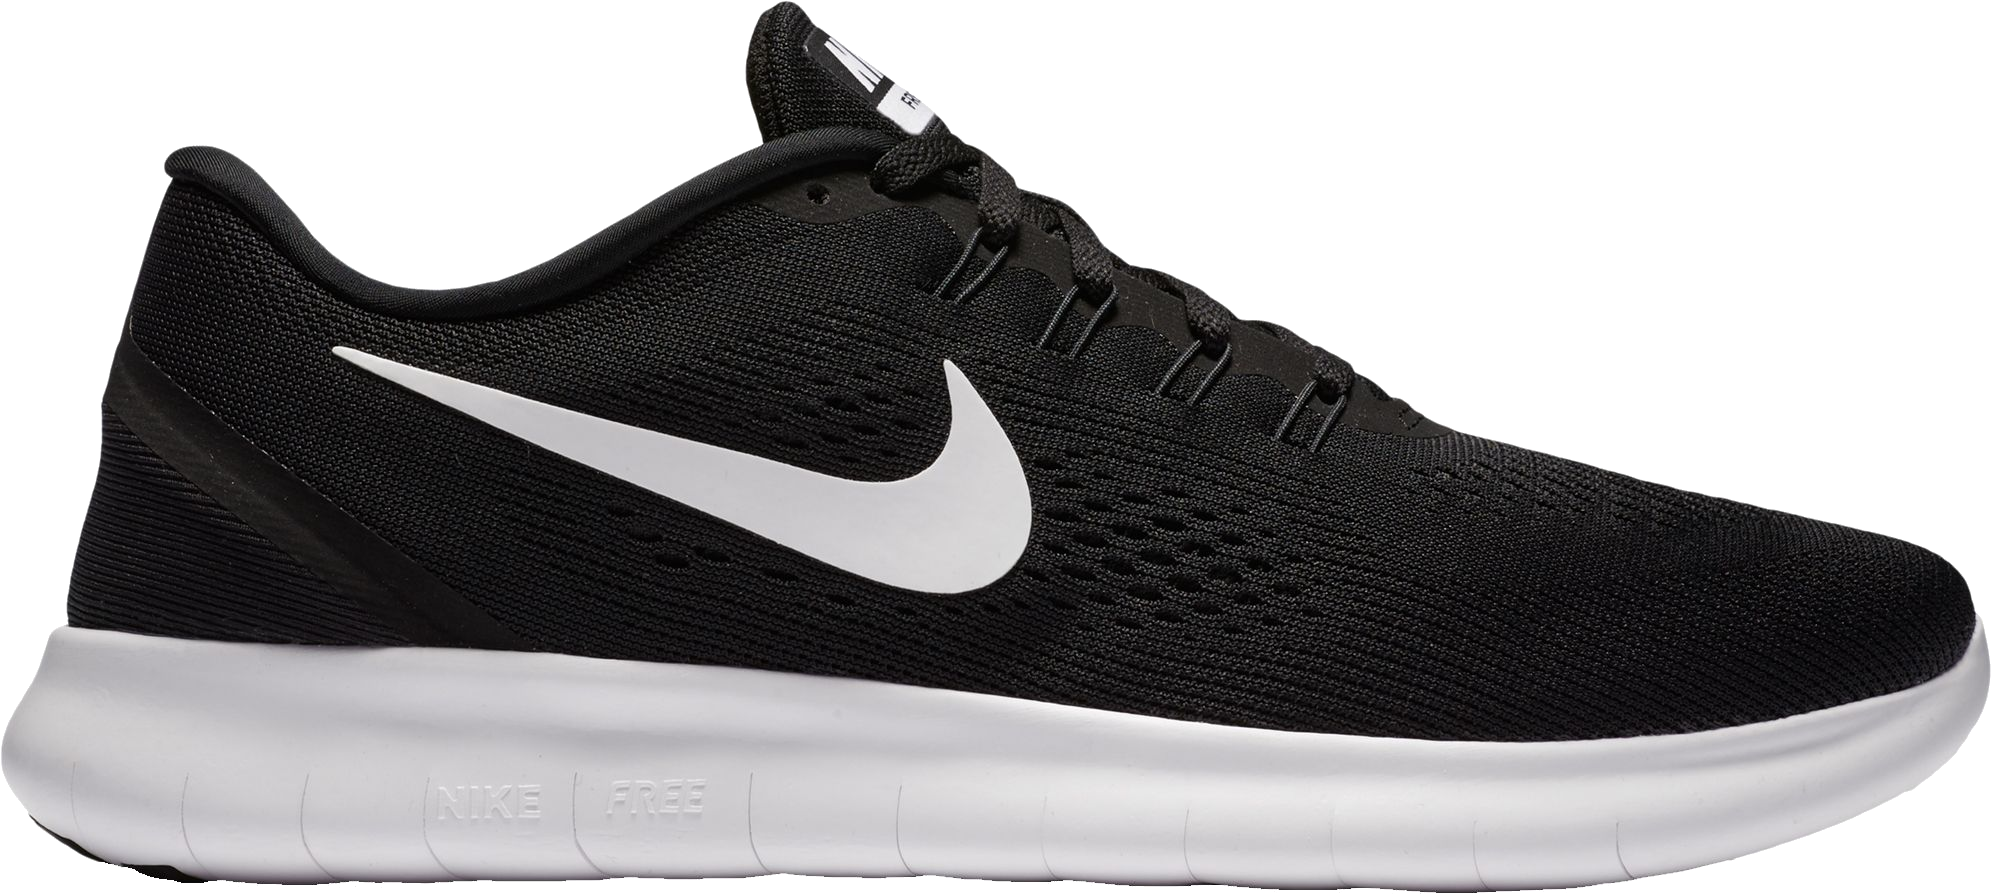
\includegraphics[scale=0.07]{../assets/nikey.png}

\section*{Data analysis}

Once the data has been collected it can be analysed and used to evaluate the project. Here are some ideas: (not all of these seem they can be used to evaluate, rather they're just interesting.)
\begin{enumerate}
	\item People playing qwop before:

	What effect did people playing qwop have on their scores, and did it skew the ability to play the original over my version? (during the first questionnaire it could assign a player into group A or B such that people who have played before are split equally between the groups to make that better statistically)
	\item Distance travelled per run

	The distance travelled can be made into graphs.
	Each user can have a plot of distance reached against the time in the test.
	Will probably increase over time.

	Can then combine them with other users onto the same graph to see how different players improve. can also see how it changes on the different versions

	\item Which game was easiest?
	The distance data can then be combined in more interesting ways. If we define the success of a user as the best distance reached during regular chunks of time, then as the data is not continuous we can compare different users in better ways. For Example this could be used to make a box plot for each section of time showing the average progress the users have made by that point in time. The data sets can also be separated for each version of the game. This can then be used to see which one was easiest overall, which one the users improved at quickest and which had greatest variation in performance of the users.

	\item Did the ordering of versions change average score?
	The data above could also be split in half again by splitting each versions into another 2 datasets; for those in group A or B (whether that game was played first or second). Then we can see how much of an effect practising on the other one first changed how far they could get.
	It could also be interesting to see the difference between the two groups in each version, which game helped the users improve at the others more.

\end{enumerate}


% 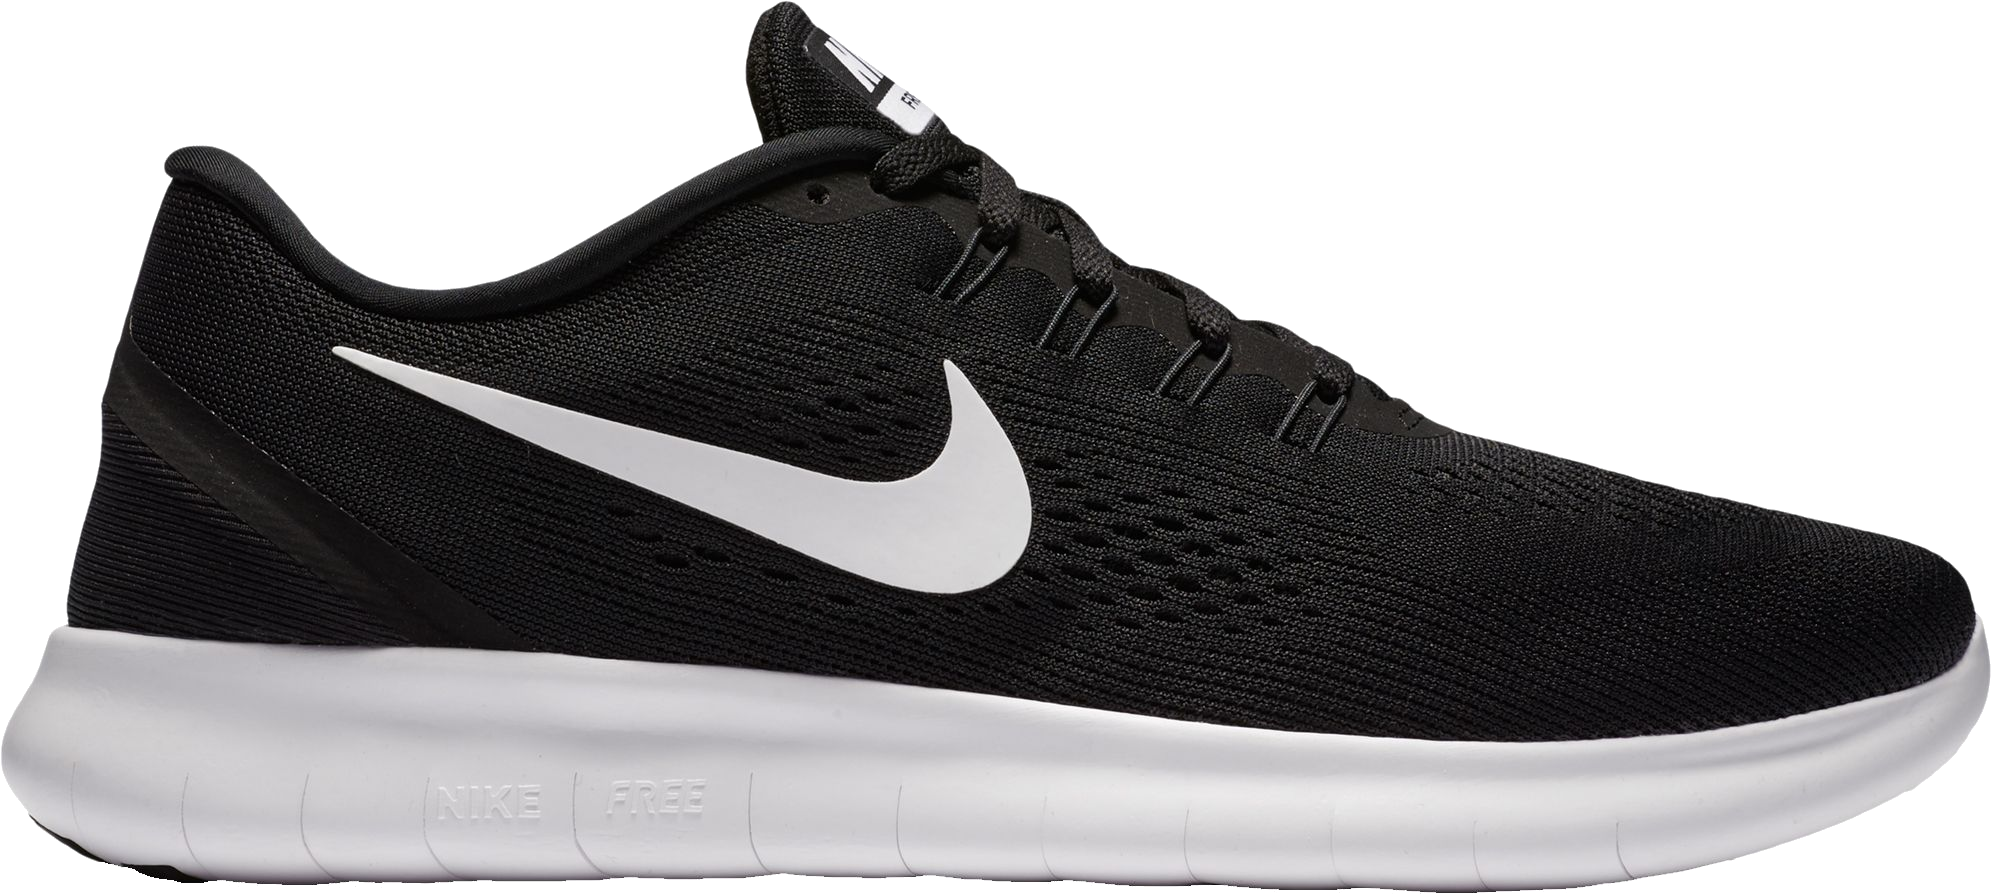
\includegraphics[scale=0.07]{../assets/nikey.png}


\end{document}